\documentclass[a4paper,oneside,12pt]{amsart}

%\usepackage[spanish, activeacute]{babel}
\usepackage[utf8]{inputenc}
%\usepackage[latin1]{inputenc}
\usepackage{latexsym}
\usepackage{multicol}
\usepackage{enumerate}
\usepackage{booktabs}
\usepackage{xcolor}
\usepackage[heightrounded]{geometry}
\geometry{top=2cm,bottom=2cm,left=2cm,right=2cm}
\usepackage{graphicx}
\usepackage{tikz}
\usepackage{tikz-network}
\usetikzlibrary{decorations.pathreplacing}

\DeclareMathOperator{\cond}{cond}
\DeclareMathOperator{\Id}{Id}
\DeclareMathOperator{\re}{Re}
%\DeclareMathOperator{\im}{Im}
\newcommand{\I}{\mathbb{I}}
\newcommand{\R}{\mathbb{R}}
\newcommand{\Q}{\mathbb{Q}}
\newcommand{\C}{\mathbb{C}}
\newcommand{\Z}{\mathbb{Z}}
\newcommand{\N}{\mathbb{N}}
\DeclareMathOperator{\im}{Im}

\newcommand{\nombremateria}
{Investigaci\'on Operativa}
\newcommand{\nombrecuatrimestre}
    {Segundo cuatrimestre de 2020}
\newcommand{\numeroparcial}
    { Tercer Parcial }
\newcommand{\fecha}
    {27 de Noviembre de 2020}
\newcommand{\numerotema}
    {\bf 1}

%\oddsidemargin -1cm \evensidemargin -1cm \textwidth 17.5cm
%topmargin 1.2cm \textheight 25cm
%\setlength{\textheight}{25cm}

\def \ds{\displaystyle}
\newtheorem{quest}{Ejercicio}
\thispagestyle{empty}

\begin{document}

\hfill \hfill
\begin{tabular}[c]{|c|c|c|c|c|c|}
\hline 
1 & 2 & 3 & 4 & 5 & Calificaci\'on \\ \hline \hline
\hspace{1 cm} & \hspace{1 cm} & \hspace{1 cm} & \hspace{1 cm} & \hspace{1 cm} & \hspace{1.3 cm} \\
\hspace{1 cm} & \hspace{1  cm} & \hspace{1  cm} & \hspace{1  cm} & \hspace{1  cm} & \hspace{1.3 cm} \\ \hline

\end{tabular}

\vspace{-1cm}

\noindent Nombre y apellido:

\vspace{0.2cm}

\noindent Número de libreta:

\noindent \hrulefill 

\smallskip
\renewcommand{\baselinestretch}{1.1}

\begin{center}
	\large \textbf{\nombremateria} 
	
	\numeroparcial -- \fecha
\end{center}

\vspace{.6cm}
\renewcommand{\theenumi}{\textbf{\arabic{enumi}}}


%%% EMPIEZA EL EJERCICIO 1 %%%
\begin{quest} 
Sea $T$ un árbol generador mínimo de un grafo pesado conexo $\mathcal{G}=(\mathbb{V}, \mathbb{E})$ y sea $\mathbb{V}'\subset \mathbb{V}$. Sea $T'$ el subgrafo de $T$ inducido por $\mathbb{V}'$ y sea $\mathcal{G}'$ el subgrafo de $\mathcal{G}$ inducido por $\mathbb{V}'$. Demostrar que si $T'$ es conexo, entonces $T'$ es un árbol generador mínimo de $\mathcal{G}'$.
\end{quest}

%%% EMPIEZA EL EJERCICIO 2 %%%
\begin{quest} 
Probar las siguientes afimaciones:
\begin{enumerate}
    \item Sea $\mathcal{G}$ un grafo conexo planar, mostrar que $\delta(\mathcal{G})\leq 5$ (es decir, existe al menos un vértice con grado menor o igual a $5$).
    \item Sean $\mathcal{G}_1=(\mathbb{V}_1, \mathbb{E}_1)$ y $\mathcal{G}_2(\mathbb{V}_2, \mathbb{E}_2)$ grafos conexos sin vértices en común. Sean $u\in \mathbb{V}_1$, $v\in \mathbb{V}_2$, $\mathcal{G}_3=(\mathbb{V}_1\cup \mathbb{V}_2, \mathbb{E}_1\cup \mathbb{E}_2\cup \{e\})$ siendo $e$ la arista que conecta a $u$ y a $v$. Mostrar que si existe un circuito euleriano en $\mathcal{G}_1$ y existe un circuito euleriano en $\mathcal{G}_2$, entonces $\mathcal{G}_3$ tiene camino euleriano y no tiene circuito euleriano.
    \item En la siguiente red de flujo, el n\'umero que acompa\~na a cada arista representa su capacidad. Demostrar que el flujo m\'aximo de $s$ a $t$ en la red es 5.
    
\begin{figure}[h!]
    \centering
    \scalebox{0.7}{
        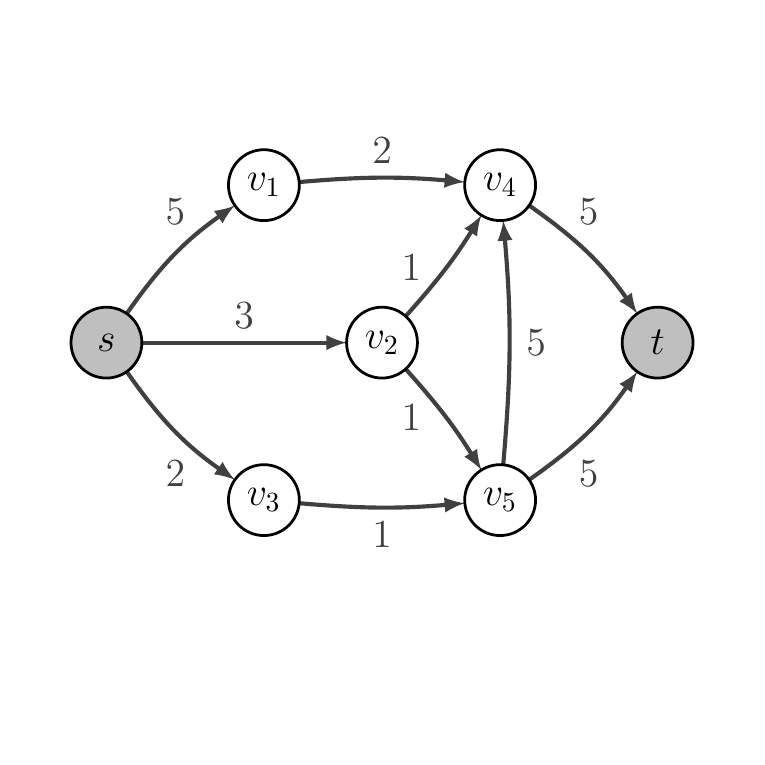
\begin{tikzpicture}
        \clip (0,0) rectangle (9.0,9.0);
        \Vertex[x=1.000,y=5.000,size=0.9,color=gray,opacity=0.5,Math,fontsize = \Large,label=s,position=center]{S}
        \Vertex[x=3.000,y=7.000,size=0.9,color=white,opacity=0.5,Math,fontsize = \Large,label=v_1,position=center]{V1}
        \Vertex[x=4.500,y=5.000,size=0.9,color=white,opacity=0.5,Math,fontsize = \Large,label=v_2,position=center]{V2}
        \Vertex[x=3.000,y=3.000,size=0.9,color=white,opacity=0.5,Math,fontsize = \Large,label=v_3,position=center]{V3}
        \Vertex[x=6.000,y=7.000,size=0.9,color=white,opacity=0.5,Math,fontsize = \Large,label=v_4,position=center]{V4}
        \Vertex[x=6.000,y=3.000,size=0.9,color=white,opacity=0.5,Math,fontsize = \Large,label=v_5,position=center]{V5}
        \Vertex[x=8.000,y=5.000,size=0.9,color=gray,opacity=0.5,Math,fontsize = \Large,label=t,position=center]{T}
        
        \Edge[label = 5, fontsize = \Large, position = {above = 3mm},lw=1.5,bend=10.000,Direct](S)(V1)
        \Edge[label = 3, fontsize = \Large, position = {above = 1mm},lw=1.5,bend=0.000,Direct](S)(V2)
        \Edge[label = 2, fontsize = \Large, position = {below = 3mm},lw=1.5,bend=-10.000,Direct](S)(V3)
        \Edge[label = 2, fontsize = \Large, position = {above = 1mm},lw=1.5,bend=5.000,Direct](V1)(V4)
        \Edge[label = 1, fontsize = \Large, position = {above = 1mm, left = 2mm},lw=1.5,bend=-5.000,Direct](V2)(V4)
        \Edge[label = 1, fontsize = \Large, position = {below = 1mm, left = 2mm},lw=1.5,bend=5.000,Direct](V2)(V5)
        \Edge[label = 1, fontsize = \Large, position = {below = 1mm},lw=1.5,bend=-5.000,Direct](V3)(V5)
        \Edge[label = 5, fontsize = \Large, position = {above = 3mm},lw=1.5,bend=10.000,Direct](V4)(T)
        \Edge[label = 5, fontsize = \Large, position = {right = 1mm},lw=1.5,bend=-5.000,Direct](V5)(V4)
        \Edge[label = 5, fontsize = \Large, position = {below = 3mm},lw=1.5,bend=-10.000,Direct](V5)(T)
        \end{tikzpicture}
    }
\end{figure}
    
\end{enumerate}
\end{quest}

%%% EMPIEZA EL EJERCICIO 3 %%%
\begin{quest}
	Mediante el algoritmo de conexión-contracción, calcular el número cromático y el polinomio cromático del siguiente grafo.
\begin{figure}[h!]
    \centering
    \scalebox{0.6}{
        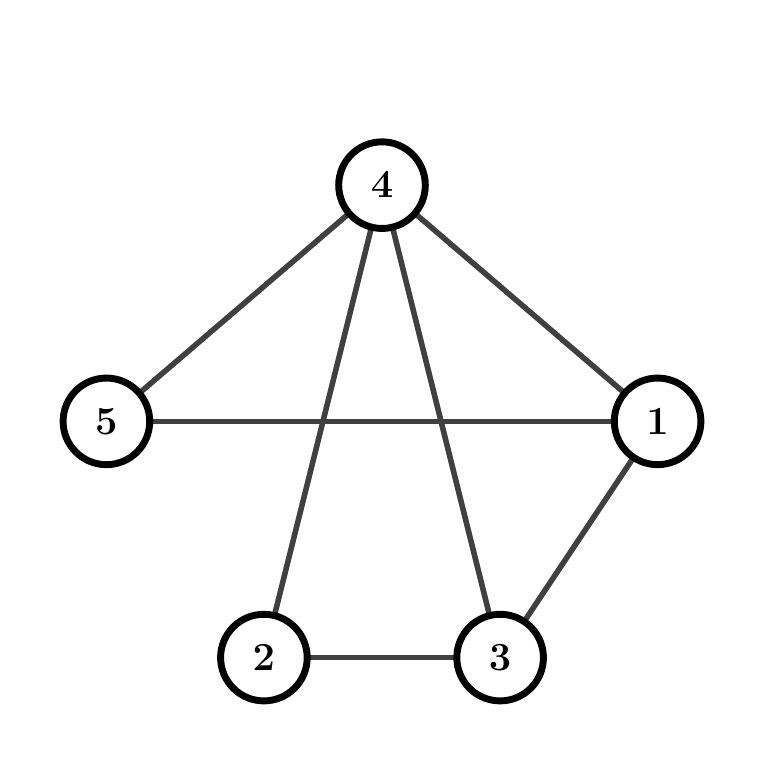
\begin{tikzpicture}
        \SetVertexStyle[LineWidth = 2.5pt]
        \clip (0,0) rectangle (9.0,9.0);
        \Vertex[x=1.000,y=4.000,size=1.1,color=white,opacity=0.5,Math,fontsize = \Large,label={\bf 5},position=center]{5}
        \Vertex[x=3.000,y=1.000,size=1.1,color=white,opacity=0.5,Math,fontsize = \Large,label={\bf 2},position=center]{2}
        \Vertex[x=6.000,y=1.000,size=1.1,color=white,opacity=0.5,Math,fontsize = \Large,label={\bf 3},position=center]{3}
        \Vertex[x=8.000,y=4.000,size=1.1,color=white,opacity=0.5,Math,fontsize = \Large,label={\bf 1},position=center]{1}
        \Vertex[x=4.500,y=7.000,size=1.1,color=white,opacity=0.5,Math,fontsize = \Large,label={\bf 4},position=center]{4}
        % \Vertex[x=7.500,y=7.000,size=1.1,color=white,opacity=0.5,Math,fontsize = \Large,label={\bf 6},position=center]{6}
        
        \Edge[lw=2.0,bend=0.000](1)(4)
        \Edge[lw=2.0,bend=0.000](1)(5)
        \Edge[lw=2.0,bend=0.000](1)(3)
        \Edge[lw=2.0,bend=0.000](2)(3)
        \Edge[lw=2.0,bend=0.000](2)(4)
        \Edge[lw=2.0,bend=0.000](3)(4)
        \Edge[lw=2.0,bend=0.000](4)(5)
        % \Edge[lw=2.0,bend=0.000](4)(6)
        
        \end{tikzpicture}
    }
\end{figure}
	%\begin{center}
	%	\includegraphics[scale=0.6]{graph.png}
	%\end{center}
% 	\boxed{\textbf{PUEDE IR CUALQUIER OTRO}}
\end{quest}

%%% EMPIEZA EL EJERCICIO 4 %%%
\begin{quest}{\tiny \hspace{1cm}}

\begin{itemize}
    \item[a)]  Un grafo es arco-circular si es el grafo intersección de arcos (abiertos) alrededor de un círculo. Un grafo es arco-circular propio si es arco-circular y tiene una representación por arcos, de modo que no haya ningún arco contenido en otro. Mostrar un ejemplo minimal de un grafo arco-circular que no sea arco-circular propio (la minimalidad quiere decir que todo subgrafo inducido sí sea arco-circular propio). Justificar la pertenencia, la no pertenencia y la minimalidad.
    
    \item[b)] Un grafo es círculo si es el grafo intersección de cuerdas dentro de un círculo. Un grafo es círculo-H si es círculo y tiene una representación por cuerdas, de modo que las cuerdas representando todo subgrafo completo tengan una intersección común. Mostrar un ejemplo minimal de un grafo círculo que no sea círculo-H. (la minimalidad quiere decir que todo subgrafo inducido sí sea círculo-H). Justificar la pertenencia, la no pertenencia y la minimalidad.
\end{itemize}
\end{quest}

\begin{quest}
En este problema se tiene un laberinto que puede representarse como un tablero de $m \times n$ ($m$ filas y $n$ columnas). Se comienza en la esquina superior izquierda y se debe alcanzar la casilla inferior derecha. En algunas casillas del laberinto puede haber puertas de color rojo o magenta, y en otras casillas del laberinto puede haber llaves de alguno de esos mismos colores. El objetivo es llegar a la salida en la menor cantidad de tiempo, pero hay algunas salvedades.

\begin{itemize}
    \item Moverse a una casilla vac\'ia cuesta \textit{1 unidad de tiempo}.
    \item No se puede mover a una casilla que tiene una puerta sin haber  \textit{agarrado} una llave del color de la puerta previamente.
    \item Solo se puede \textit{agarrar una llave} estando en la casilla donde se ubica una llave, para lo cual se tardan \textit{5 unidades de tiempo}.
\end{itemize}

\begin{center}
    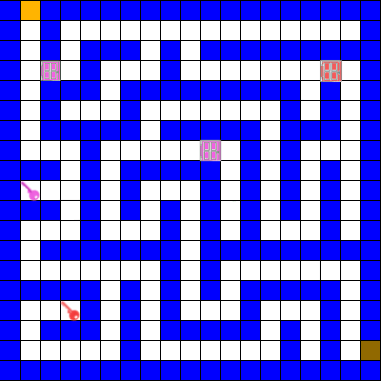
\includegraphics[scale = 0.5]{laberinto.png}    
\end{center}

Teniendo esto en cuenta, se pide:

\begin{enumerate}
    \item Modelar el problema como un problema de grafos y proponer un algoritmo que utilice dicho grafo para resolver el problema. ¿Cuál es la complejidad? Expresarla en términos de $m$ y $n$.
    \item ¿C\'omo se modificar\'ia la complejidad si ahora se tienen $k$ colores posibles de llaves y puertas? Expresarla en términos de $m$, $n$ y $k$.
\end{enumerate}

{\bf Sugerencia}: Puede ser necesario considerar m\'as que un nodo por casilla del tablero, para tener en cuenta adem\'as qu\'e llaves se poseen.
\end{quest}

% \hline



% \medskip
% \begin{quest}
% 	Probar que para todo grafo $\mathcal{G}$ de $n$ v\'ertices vale que $\chi{\mathcal{G}}\cdot \chi({\bar{\mathcal{G}}}) \geq n$.
% 	\medskip
	
% 	\textbf{Sugerencia/Observaci\'on}: $\mathcal{G} \cup \mathcal{\bar{G}} = K_n$ 
% \end{quest}

% \begin{quest}
% 	Sea $\mathcal{G}$ un grafo de $2n$ v\'ertices, todos ellos con grado al menos $n$. Probar que $\mathcal{G}$ tiene un matching perfecto.
% \end{quest}


% \begin{quest}
% 	Un grafo completo orientado (entre todo par de v\'ertices hay exactamente una arista en alguna direcci\'on) se lo conoce con el nombre de $\textit{grafo torneo}$. Probar que todo grafo torneo contiene un camino hamiltoniano (dirigido).
	
% 	\textbf{Sugerencia}: Puede utilizar inducci\'on para probar el resultado.
% \end{quest}



% \begin{quest} 
% 	Sean $a_1, \dots, a_{2n}$ n\'umeros enteros mayores o iguales que 2. Se desea armar la mayor cantidad de parejas $(a_i,a_j), i \neq j$ (cada $a_i$ puede estar en a lo sumo una pareja).
		
% 	Modelar el problema en t\'erminos de teor\'ia de grafos, de forma de poder resolverlo mediante alg\'un algoritmo visto en clase.
% \end{quest}





%%% TERMINA EL PARCIAL %%%



\end{document}

